% Created by tikzDevice version 0.12 on 2019-01-03 18:24:26
% !TEX encoding = UTF-8 Unicode
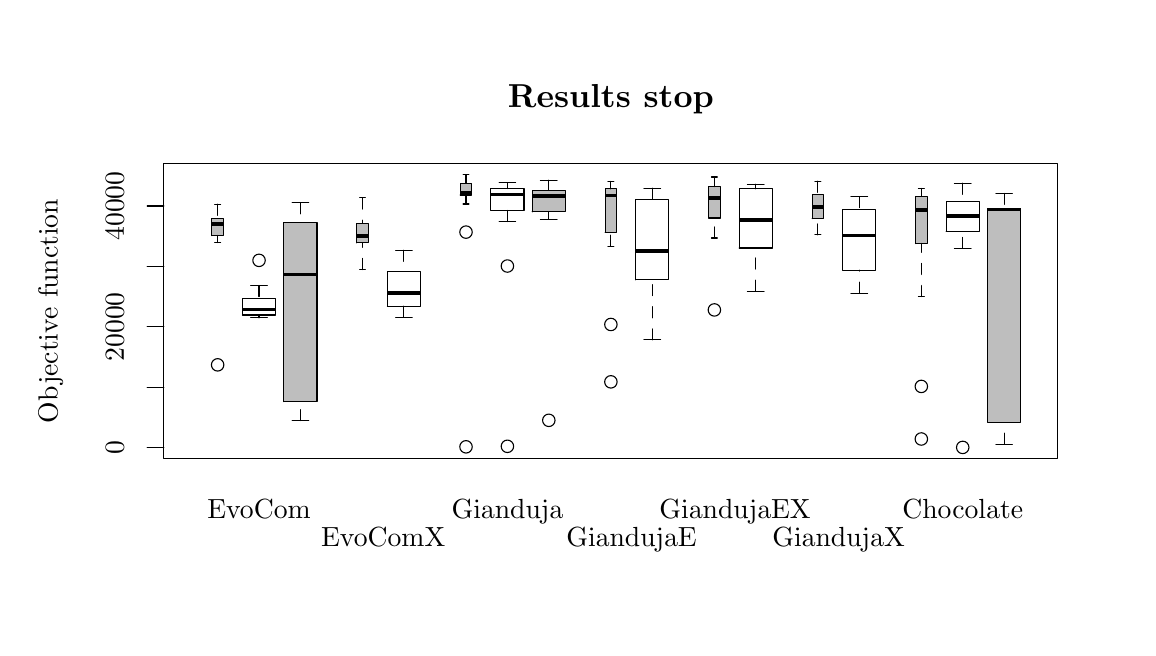
\begin{tikzpicture}[x=1pt,y=1pt]
\definecolor{fillColor}{RGB}{255,255,255}
\path[use as bounding box,fill=fillColor,fill opacity=0.00] (0,0) rectangle (397.48,216.81);
\begin{scope}
\path[clip] ( 49.20, 61.20) rectangle (372.28,167.61);
\definecolor{fillColor}{RGB}{190,190,190}

\path[fill=fillColor] ( 66.55,141.70) --
	( 70.74,141.70) --
	( 70.74,147.90) --
	( 66.55,147.90) --
	cycle;
\definecolor{drawColor}{RGB}{0,0,0}

\path[draw=drawColor,line width= 1.2pt,line join=round] ( 66.55,145.89) -- ( 70.74,145.89);

\path[draw=drawColor,line width= 0.4pt,dash pattern=on 4pt off 4pt ,line join=round,line cap=round] ( 68.64,139.16) -- ( 68.64,141.70);

\path[draw=drawColor,line width= 0.4pt,dash pattern=on 4pt off 4pt ,line join=round,line cap=round] ( 68.64,153.00) -- ( 68.64,147.90);

\path[draw=drawColor,line width= 0.4pt,line join=round,line cap=round] ( 67.60,139.16) -- ( 69.69,139.16);

\path[draw=drawColor,line width= 0.4pt,line join=round,line cap=round] ( 67.60,153.00) -- ( 69.69,153.00);

\path[draw=drawColor,line width= 0.4pt,line join=round,line cap=round] ( 66.55,141.70) --
	( 70.74,141.70) --
	( 70.74,147.90) --
	( 66.55,147.90) --
	( 66.55,141.70);

\path[draw=drawColor,line width= 0.4pt,line join=round,line cap=round] ( 68.64, 94.97) circle (  2.25);
\definecolor{fillColor}{RGB}{255,255,255}

\path[fill=fillColor] ( 77.62,113.00) --
	( 89.59,113.00) --
	( 89.59,118.79) --
	( 77.62,118.79) --
	cycle;

\path[draw=drawColor,line width= 1.2pt,line join=round] ( 77.62,114.90) -- ( 89.59,114.90);

\path[draw=drawColor,line width= 0.4pt,dash pattern=on 4pt off 4pt ,line join=round,line cap=round] ( 83.60,111.98) -- ( 83.60,113.00);

\path[draw=drawColor,line width= 0.4pt,dash pattern=on 4pt off 4pt ,line join=round,line cap=round] ( 83.60,123.66) -- ( 83.60,118.79);

\path[draw=drawColor,line width= 0.4pt,line join=round,line cap=round] ( 80.61,111.98) -- ( 86.59,111.98);

\path[draw=drawColor,line width= 0.4pt,line join=round,line cap=round] ( 80.61,123.66) -- ( 86.59,123.66);

\path[draw=drawColor,line width= 0.4pt,line join=round,line cap=round] ( 77.62,113.00) --
	( 89.59,113.00) --
	( 89.59,118.79) --
	( 77.62,118.79) --
	( 77.62,113.00);

\path[draw=drawColor,line width= 0.4pt,line join=round,line cap=round] ( 83.60,132.73) circle (  2.25);
\definecolor{fillColor}{RGB}{190,190,190}

\path[fill=fillColor] ( 92.58, 81.66) --
	(104.54, 81.66) --
	(104.54,146.35) --
	( 92.58,146.35) --
	cycle;

\path[draw=drawColor,line width= 1.2pt,line join=round] ( 92.58,127.64) -- (104.54,127.64);

\path[draw=drawColor,line width= 0.4pt,dash pattern=on 4pt off 4pt ,line join=round,line cap=round] ( 98.56, 74.80) -- ( 98.56, 81.66);

\path[draw=drawColor,line width= 0.4pt,dash pattern=on 4pt off 4pt ,line join=round,line cap=round] ( 98.56,153.54) -- ( 98.56,146.35);

\path[draw=drawColor,line width= 0.4pt,line join=round,line cap=round] ( 95.57, 74.80) -- (101.55, 74.80);

\path[draw=drawColor,line width= 0.4pt,line join=round,line cap=round] ( 95.57,153.54) -- (101.55,153.54);

\path[draw=drawColor,line width= 0.4pt,line join=round,line cap=round] ( 92.58, 81.66) --
	(104.54, 81.66) --
	(104.54,146.35) --
	( 92.58,146.35) --
	( 92.58, 81.66);

\path[fill=fillColor] (118.90,139.04) --
	(123.09,139.04) --
	(123.09,146.15) --
	(118.90,146.15) --
	cycle;

\path[draw=drawColor,line width= 1.2pt,line join=round] (118.90,141.51) -- (123.09,141.51);

\path[draw=drawColor,line width= 0.4pt,dash pattern=on 4pt off 4pt ,line join=round,line cap=round] (121.00,129.42) -- (121.00,139.04);

\path[draw=drawColor,line width= 0.4pt,dash pattern=on 4pt off 4pt ,line join=round,line cap=round] (121.00,155.28) -- (121.00,146.15);

\path[draw=drawColor,line width= 0.4pt,line join=round,line cap=round] (119.95,129.42) -- (122.04,129.42);

\path[draw=drawColor,line width= 0.4pt,line join=round,line cap=round] (119.95,155.28) -- (122.04,155.28);

\path[draw=drawColor,line width= 0.4pt,line join=round,line cap=round] (118.90,139.04) --
	(123.09,139.04) --
	(123.09,146.15) --
	(118.90,146.15) --
	(118.90,139.04);
\definecolor{fillColor}{RGB}{255,255,255}

\path[fill=fillColor] (129.97,116.16) --
	(141.94,116.16) --
	(141.94,128.54) --
	(129.97,128.54) --
	cycle;

\path[draw=drawColor,line width= 1.2pt,line join=round] (129.97,120.91) -- (141.94,120.91);

\path[draw=drawColor,line width= 0.4pt,dash pattern=on 4pt off 4pt ,line join=round,line cap=round] (135.95,112.20) -- (135.95,116.16);

\path[draw=drawColor,line width= 0.4pt,dash pattern=on 4pt off 4pt ,line join=round,line cap=round] (135.95,136.37) -- (135.95,128.54);

\path[draw=drawColor,line width= 0.4pt,line join=round,line cap=round] (132.96,112.20) -- (138.95,112.20);

\path[draw=drawColor,line width= 0.4pt,line join=round,line cap=round] (132.96,136.37) -- (138.95,136.37);

\path[draw=drawColor,line width= 0.4pt,line join=round,line cap=round] (129.97,116.16) --
	(141.94,116.16) --
	(141.94,128.54) --
	(129.97,128.54) --
	(129.97,116.16);
\definecolor{fillColor}{RGB}{190,190,190}

\path[fill=fillColor] (156.30,156.33) --
	(160.48,156.33) --
	(160.48,160.64) --
	(156.30,160.64) --
	cycle;

\path[draw=drawColor,line width= 1.2pt,line join=round] (156.30,157.22) -- (160.48,157.22);

\path[draw=drawColor,line width= 0.4pt,dash pattern=on 4pt off 4pt ,line join=round,line cap=round] (158.39,153.11) -- (158.39,156.33);

\path[draw=drawColor,line width= 0.4pt,dash pattern=on 4pt off 4pt ,line join=round,line cap=round] (158.39,163.67) -- (158.39,160.64);

\path[draw=drawColor,line width= 0.4pt,line join=round,line cap=round] (157.34,153.11) -- (159.44,153.11);

\path[draw=drawColor,line width= 0.4pt,line join=round,line cap=round] (157.34,163.67) -- (159.44,163.67);

\path[draw=drawColor,line width= 0.4pt,line join=round,line cap=round] (156.30,156.33) --
	(160.48,156.33) --
	(160.48,160.64) --
	(156.30,160.64) --
	(156.30,156.33);

\path[draw=drawColor,line width= 0.4pt,line join=round,line cap=round] (158.39,142.94) circle (  2.25);

\path[draw=drawColor,line width= 0.4pt,line join=round,line cap=round] (158.39, 65.35) circle (  2.25);
\definecolor{fillColor}{RGB}{255,255,255}

\path[fill=fillColor] (167.37,150.83) --
	(179.33,150.83) --
	(179.33,158.65) --
	(167.37,158.65) --
	cycle;

\path[draw=drawColor,line width= 1.2pt,line join=round] (167.37,156.46) -- (179.33,156.46);

\path[draw=drawColor,line width= 0.4pt,dash pattern=on 4pt off 4pt ,line join=round,line cap=round] (173.35,146.75) -- (173.35,150.83);

\path[draw=drawColor,line width= 0.4pt,dash pattern=on 4pt off 4pt ,line join=round,line cap=round] (173.35,160.80) -- (173.35,158.65);

\path[draw=drawColor,line width= 0.4pt,line join=round,line cap=round] (170.36,146.75) -- (176.34,146.75);

\path[draw=drawColor,line width= 0.4pt,line join=round,line cap=round] (170.36,160.80) -- (176.34,160.80);

\path[draw=drawColor,line width= 0.4pt,line join=round,line cap=round] (167.37,150.83) --
	(179.33,150.83) --
	(179.33,158.65) --
	(167.37,158.65) --
	(167.37,150.83);

\path[draw=drawColor,line width= 0.4pt,line join=round,line cap=round] (173.35,130.68) circle (  2.25);

\path[draw=drawColor,line width= 0.4pt,line join=round,line cap=round] (173.35, 65.54) circle (  2.25);
\definecolor{fillColor}{RGB}{190,190,190}

\path[fill=fillColor] (182.32,150.23) --
	(194.29,150.23) --
	(194.29,158.05) --
	(182.32,158.05) --
	cycle;

\path[draw=drawColor,line width= 1.2pt,line join=round] (182.32,156.00) -- (194.29,156.00);

\path[draw=drawColor,line width= 0.4pt,dash pattern=on 4pt off 4pt ,line join=round,line cap=round] (188.31,147.53) -- (188.31,150.23);

\path[draw=drawColor,line width= 0.4pt,dash pattern=on 4pt off 4pt ,line join=round,line cap=round] (188.31,161.70) -- (188.31,158.05);

\path[draw=drawColor,line width= 0.4pt,line join=round,line cap=round] (185.31,147.53) -- (191.30,147.53);

\path[draw=drawColor,line width= 0.4pt,line join=round,line cap=round] (185.31,161.70) -- (191.30,161.70);

\path[draw=drawColor,line width= 0.4pt,line join=round,line cap=round] (182.32,150.23) --
	(194.29,150.23) --
	(194.29,158.05) --
	(182.32,158.05) --
	(182.32,150.23);

\path[draw=drawColor,line width= 0.4pt,line join=round,line cap=round] (188.31, 74.93) circle (  2.25);

\path[fill=fillColor] (208.65,142.87) --
	(212.84,142.87) --
	(212.84,158.54) --
	(208.65,158.54) --
	cycle;

\path[draw=drawColor,line width= 1.2pt,line join=round] (208.65,156.19) -- (212.84,156.19);

\path[draw=drawColor,line width= 0.4pt,dash pattern=on 4pt off 4pt ,line join=round,line cap=round] (210.74,137.82) -- (210.74,142.87);

\path[draw=drawColor,line width= 0.4pt,dash pattern=on 4pt off 4pt ,line join=round,line cap=round] (210.74,161.25) -- (210.74,158.54);

\path[draw=drawColor,line width= 0.4pt,line join=round,line cap=round] (209.70,137.82) -- (211.79,137.82);

\path[draw=drawColor,line width= 0.4pt,line join=round,line cap=round] (209.70,161.25) -- (211.79,161.25);

\path[draw=drawColor,line width= 0.4pt,line join=round,line cap=round] (208.65,142.87) --
	(212.84,142.87) --
	(212.84,158.54) --
	(208.65,158.54) --
	(208.65,142.87);

\path[draw=drawColor,line width= 0.4pt,line join=round,line cap=round] (210.74, 88.83) circle (  2.25);

\path[draw=drawColor,line width= 0.4pt,line join=round,line cap=round] (210.74,109.56) circle (  2.25);
\definecolor{fillColor}{RGB}{255,255,255}

\path[fill=fillColor] (219.72,125.72) --
	(231.68,125.72) --
	(231.68,154.56) --
	(219.72,154.56) --
	cycle;

\path[draw=drawColor,line width= 1.2pt,line join=round] (219.72,136.13) -- (231.68,136.13);

\path[draw=drawColor,line width= 0.4pt,dash pattern=on 4pt off 4pt ,line join=round,line cap=round] (225.70,103.98) -- (225.70,125.72);

\path[draw=drawColor,line width= 0.4pt,dash pattern=on 4pt off 4pt ,line join=round,line cap=round] (225.70,158.80) -- (225.70,154.56);

\path[draw=drawColor,line width= 0.4pt,line join=round,line cap=round] (222.71,103.98) -- (228.69,103.98);

\path[draw=drawColor,line width= 0.4pt,line join=round,line cap=round] (222.71,158.80) -- (228.69,158.80);

\path[draw=drawColor,line width= 0.4pt,line join=round,line cap=round] (219.72,125.72) --
	(231.68,125.72) --
	(231.68,154.56) --
	(219.72,154.56) --
	(219.72,125.72);
\definecolor{fillColor}{RGB}{190,190,190}

\path[fill=fillColor] (246.04,148.04) --
	(250.23,148.04) --
	(250.23,159.40) --
	(246.04,159.40) --
	cycle;

\path[draw=drawColor,line width= 1.2pt,line join=round] (246.04,155.25) -- (250.23,155.25);

\path[draw=drawColor,line width= 0.4pt,dash pattern=on 4pt off 4pt ,line join=round,line cap=round] (248.14,140.80) -- (248.14,148.04);

\path[draw=drawColor,line width= 0.4pt,dash pattern=on 4pt off 4pt ,line join=round,line cap=round] (248.14,162.84) -- (248.14,159.40);

\path[draw=drawColor,line width= 0.4pt,line join=round,line cap=round] (247.09,140.80) -- (249.18,140.80);

\path[draw=drawColor,line width= 0.4pt,line join=round,line cap=round] (247.09,162.84) -- (249.18,162.84);

\path[draw=drawColor,line width= 0.4pt,line join=round,line cap=round] (246.04,148.04) --
	(250.23,148.04) --
	(250.23,159.40) --
	(246.04,159.40) --
	(246.04,148.04);

\path[draw=drawColor,line width= 0.4pt,line join=round,line cap=round] (248.14,114.82) circle (  2.25);
\definecolor{fillColor}{RGB}{255,255,255}

\path[fill=fillColor] (257.11,137.18) --
	(269.08,137.18) --
	(269.08,158.54) --
	(257.11,158.54) --
	cycle;

\path[draw=drawColor,line width= 1.2pt,line join=round] (257.11,147.35) -- (269.08,147.35);

\path[draw=drawColor,line width= 0.4pt,dash pattern=on 4pt off 4pt ,line join=round,line cap=round] (263.09,121.58) -- (263.09,137.18);

\path[draw=drawColor,line width= 0.4pt,dash pattern=on 4pt off 4pt ,line join=round,line cap=round] (263.09,160.22) -- (263.09,158.54);

\path[draw=drawColor,line width= 0.4pt,line join=round,line cap=round] (260.10,121.58) -- (266.09,121.58);

\path[draw=drawColor,line width= 0.4pt,line join=round,line cap=round] (260.10,160.22) -- (266.09,160.22);

\path[draw=drawColor,line width= 0.4pt,line join=round,line cap=round] (257.11,137.18) --
	(269.08,137.18) --
	(269.08,158.54) --
	(257.11,158.54) --
	(257.11,137.18);
\definecolor{fillColor}{RGB}{190,190,190}

\path[fill=fillColor] (283.44,147.80) --
	(287.62,147.80) --
	(287.62,156.44) --
	(283.44,156.44) --
	cycle;

\path[draw=drawColor,line width= 1.2pt,line join=round] (283.44,152.01) -- (287.62,152.01);

\path[draw=drawColor,line width= 0.4pt,dash pattern=on 4pt off 4pt ,line join=round,line cap=round] (285.53,141.91) -- (285.53,147.80);

\path[draw=drawColor,line width= 0.4pt,dash pattern=on 4pt off 4pt ,line join=round,line cap=round] (285.53,161.34) -- (285.53,156.44);

\path[draw=drawColor,line width= 0.4pt,line join=round,line cap=round] (284.48,141.91) -- (286.58,141.91);

\path[draw=drawColor,line width= 0.4pt,line join=round,line cap=round] (284.48,161.34) -- (286.58,161.34);

\path[draw=drawColor,line width= 0.4pt,line join=round,line cap=round] (283.44,147.80) --
	(287.62,147.80) --
	(287.62,156.44) --
	(283.44,156.44) --
	(283.44,147.80);
\definecolor{fillColor}{RGB}{255,255,255}

\path[fill=fillColor] (294.51,129.20) --
	(306.47,129.20) --
	(306.47,151.11) --
	(294.51,151.11) --
	cycle;

\path[draw=drawColor,line width= 1.2pt,line join=round] (294.51,141.65) -- (306.47,141.65);

\path[draw=drawColor,line width= 0.4pt,dash pattern=on 4pt off 4pt ,line join=round,line cap=round] (300.49,120.87) -- (300.49,129.20);

\path[draw=drawColor,line width= 0.4pt,dash pattern=on 4pt off 4pt ,line join=round,line cap=round] (300.49,155.78) -- (300.49,151.11);

\path[draw=drawColor,line width= 0.4pt,line join=round,line cap=round] (297.50,120.87) -- (303.48,120.87);

\path[draw=drawColor,line width= 0.4pt,line join=round,line cap=round] (297.50,155.78) -- (303.48,155.78);

\path[draw=drawColor,line width= 0.4pt,line join=round,line cap=round] (294.51,129.20) --
	(306.47,129.20) --
	(306.47,151.11) --
	(294.51,151.11) --
	(294.51,129.20);
\definecolor{fillColor}{RGB}{190,190,190}

\path[fill=fillColor] (320.83,138.81) --
	(325.02,138.81) --
	(325.02,155.86) --
	(320.83,155.86) --
	cycle;

\path[draw=drawColor,line width= 1.2pt,line join=round] (320.83,150.95) -- (325.02,150.95);

\path[draw=drawColor,line width= 0.4pt,dash pattern=on 4pt off 4pt ,line join=round,line cap=round] (322.92,119.63) -- (322.92,138.81);

\path[draw=drawColor,line width= 0.4pt,dash pattern=on 4pt off 4pt ,line join=round,line cap=round] (322.92,158.76) -- (322.92,155.86);

\path[draw=drawColor,line width= 0.4pt,line join=round,line cap=round] (321.88,119.63) -- (323.97,119.63);

\path[draw=drawColor,line width= 0.4pt,line join=round,line cap=round] (321.88,158.76) -- (323.97,158.76);

\path[draw=drawColor,line width= 0.4pt,line join=round,line cap=round] (320.83,138.81) --
	(325.02,138.81) --
	(325.02,155.86) --
	(320.83,155.86) --
	(320.83,138.81);

\path[draw=drawColor,line width= 0.4pt,line join=round,line cap=round] (322.92, 87.18) circle (  2.25);

\path[draw=drawColor,line width= 0.4pt,line join=round,line cap=round] (322.92, 68.18) circle (  2.25);
\definecolor{fillColor}{RGB}{255,255,255}

\path[fill=fillColor] (331.90,143.25) --
	(343.87,143.25) --
	(343.87,154.10) --
	(331.90,154.10) --
	cycle;

\path[draw=drawColor,line width= 1.2pt,line join=round] (331.90,148.80) -- (343.87,148.80);

\path[draw=drawColor,line width= 0.4pt,dash pattern=on 4pt off 4pt ,line join=round,line cap=round] (337.88,137.04) -- (337.88,143.25);

\path[draw=drawColor,line width= 0.4pt,dash pattern=on 4pt off 4pt ,line join=round,line cap=round] (337.88,160.62) -- (337.88,154.10);

\path[draw=drawColor,line width= 0.4pt,line join=round,line cap=round] (334.89,137.04) -- (340.87,137.04);

\path[draw=drawColor,line width= 0.4pt,line join=round,line cap=round] (334.89,160.62) -- (340.87,160.62);

\path[draw=drawColor,line width= 0.4pt,line join=round,line cap=round] (331.90,143.25) --
	(343.87,143.25) --
	(343.87,154.10) --
	(331.90,154.10) --
	(331.90,143.25);

\path[draw=drawColor,line width= 0.4pt,line join=round,line cap=round] (337.88, 65.14) circle (  2.25);
\definecolor{fillColor}{RGB}{190,190,190}

\path[fill=fillColor] (346.86, 74.25) --
	(358.82, 74.25) --
	(358.82,151.45) --
	(346.86,151.45) --
	cycle;

\path[draw=drawColor,line width= 1.2pt,line join=round] (346.86,151.12) -- (358.82,151.12);

\path[draw=drawColor,line width= 0.4pt,dash pattern=on 4pt off 4pt ,line join=round,line cap=round] (352.84, 66.28) -- (352.84, 74.25);

\path[draw=drawColor,line width= 0.4pt,dash pattern=on 4pt off 4pt ,line join=round,line cap=round] (352.84,156.93) -- (352.84,151.45);

\path[draw=drawColor,line width= 0.4pt,line join=round,line cap=round] (349.85, 66.28) -- (355.83, 66.28);

\path[draw=drawColor,line width= 0.4pt,line join=round,line cap=round] (349.85,156.93) -- (355.83,156.93);

\path[draw=drawColor,line width= 0.4pt,line join=round,line cap=round] (346.86, 74.25) --
	(358.82, 74.25) --
	(358.82,151.45) --
	(346.86,151.45) --
	(346.86, 74.25);
\end{scope}
\begin{scope}
\path[clip] (  0.00,  0.00) rectangle (397.48,216.81);
\definecolor{drawColor}{RGB}{0,0,0}

\node[text=drawColor,rotate= 90.00,anchor=base,inner sep=0pt, outer sep=0pt, scale=  1.00] at ( 10.80,114.41) {Objective function};
\end{scope}
\begin{scope}
\path[clip] (  0.00,  0.00) rectangle (397.48,216.81);
\definecolor{drawColor}{RGB}{0,0,0}

\node[text=drawColor,anchor=base,inner sep=0pt, outer sep=0pt, scale=  1.00] at ( 83.60, 39.60) {EvoCom};

\node[text=drawColor,anchor=base,inner sep=0pt, outer sep=0pt, scale=  1.00] at (173.35, 39.60) {Gianduja};

\node[text=drawColor,anchor=base,inner sep=0pt, outer sep=0pt, scale=  1.00] at (255.62, 39.60) {GiandujaEX};

\node[text=drawColor,anchor=base,inner sep=0pt, outer sep=0pt, scale=  1.00] at (337.88, 39.60) {Chocolate};

\node[text=drawColor,anchor=base,inner sep=0pt, outer sep=0pt, scale=  1.00] at (128.48, 29.27) {EvoComX};

\node[text=drawColor,anchor=base,inner sep=0pt, outer sep=0pt, scale=  1.00] at (218.22, 29.27) {GiandujaE};

\node[text=drawColor,anchor=base,inner sep=0pt, outer sep=0pt, scale=  1.00] at (293.01, 29.27) {GiandujaX};
\end{scope}
\begin{scope}
\path[clip] (  0.00,  0.00) rectangle (397.48,216.81);
\definecolor{drawColor}{RGB}{0,0,0}

\node[text=drawColor,anchor=base,inner sep=0pt, outer sep=0pt, scale=  1.20] at (210.74,188.07) {\bfseries Results stop};
\end{scope}
\begin{scope}
\path[clip] (  0.00,  0.00) rectangle (397.48,216.81);
\definecolor{drawColor}{RGB}{0,0,0}

\path[draw=drawColor,line width= 0.4pt,line join=round,line cap=round] ( 49.20, 65.01) -- ( 49.20,152.35);

\path[draw=drawColor,line width= 0.4pt,line join=round,line cap=round] ( 49.20, 65.01) -- ( 43.20, 65.01);

\path[draw=drawColor,line width= 0.4pt,line join=round,line cap=round] ( 49.20, 86.84) -- ( 43.20, 86.84);

\path[draw=drawColor,line width= 0.4pt,line join=round,line cap=round] ( 49.20,108.68) -- ( 43.20,108.68);

\path[draw=drawColor,line width= 0.4pt,line join=round,line cap=round] ( 49.20,130.51) -- ( 43.20,130.51);

\path[draw=drawColor,line width= 0.4pt,line join=round,line cap=round] ( 49.20,152.35) -- ( 43.20,152.35);

\node[text=drawColor,rotate= 90.00,anchor=base,inner sep=0pt, outer sep=0pt, scale=  1.00] at ( 34.80, 65.01) {0};

\node[text=drawColor,rotate= 90.00,anchor=base,inner sep=0pt, outer sep=0pt, scale=  1.00] at ( 34.80,108.68) {20000};

\node[text=drawColor,rotate= 90.00,anchor=base,inner sep=0pt, outer sep=0pt, scale=  1.00] at ( 34.80,152.35) {40000};

\path[draw=drawColor,line width= 0.4pt,line join=round,line cap=round] ( 49.20, 61.20) --
	(372.28, 61.20) --
	(372.28,167.61) --
	( 49.20,167.61) --
	( 49.20, 61.20);
\end{scope}
\end{tikzpicture}
